% !TEX root = ../Thesis.tex

\chapter{Supplementary Implementation and Evaluation Material}
\label{app:supplementary-material}

\section{Software Tools and the Use of AI Tools}

Several software tools were used during the development of the artefact and the writing of the thesis.

Codex was used as a supportive tool during development, mainly for exploring implementation alternatives, discussing frontend-backend interactions, and assisting with SQL, API logic, and debugging. While it helped improve efficiency, all system design decisions and final implementations were made by the author.

ChatGPT was used during the writing process to refine language, improve clarity, and adjust phrasing to a more academic style. As English is not the author's first language, it was particularly useful for improving grammar and sentence structure. However, all ideas and conclusions were developed independently.

Visual Studio Code served as the main development environment, draw.io was used for diagrams, and Overleaf was used for writing and formatting the thesis in \LaTeX. These tools supported the development and documentation process but did not influence the research direction or results.

\section{Detailed Implementation Notes}

The prototype was implemented as a full-stack web application in which frontend actions trigger backend workflow execution through API-based processing. The implementation followed an incremental structure: authentication, routing, CSV upload, database persistence, and intermediate report generation were implemented first, after which workflow-specific calculation stages were added. This made it possible to validate each part of the execution chain separately before integrating them into the full workflow.

The frontend was implemented using React, TypeScript, Vite, and React Router. Each workflow stage is represented through route-level pages that allow users to upload data, trigger processing, inspect intermediate results, and store snapshots. The frontend does not execute workflow logic directly. Instead, it acts as an orchestration and inspection layer by sending requests to the backend through a dedicated API client and rendering the structured responses returned by backend services.

\begin{figure}[H]
    \centering
    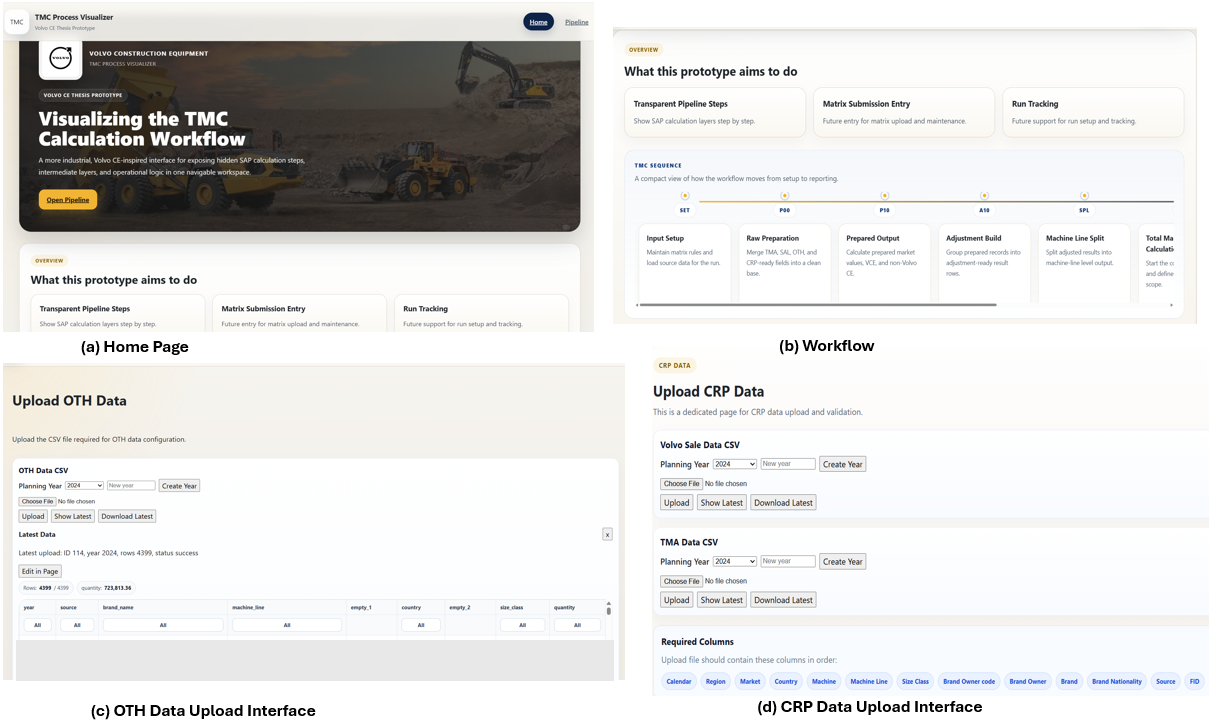
\includegraphics[width=1.1\linewidth]{5.3.1.png}
    \caption{Selected frontend views developed during the implementation of the prototype}
    \label{fig:appendix-frontend-views}
\end{figure}

The backend was implemented with Python and FastAPI. FastAPI endpoints serve as execution entry points for upload, report generation, snapshot persistence, and result retrieval. The persistence layer uses a relational database backend with environment-based switching between SQLite and PostgreSQL. During application startup, both workflow and authentication schemas are initialized before the API routes become available to the frontend.

CSV upload was implemented as the first execution stage. A user uploads a file through the frontend and selects a dataset type. The backend then routes the request to a dataset-specific handler, which parses the CSV file using \texttt{pandas}, normalizes heterogeneous input formats into a common row structure, and stores the cleaned rows in dataset-specific database tables. Upload metadata, including dataset type, planning year, upload status, and timestamp, is stored separately to support later retrieval of the latest successful input for each dataset.

Once persistence was established, source-level report generation was introduced. In this stage, backend endpoints execute SQL queries against the stored upload tables. These queries join uploaded data with mapping and control tables, such as country-group mappings, brand mappings, machine-line mappings, source matrices, and reporter lists. The purpose of these transformations is to align source data into a common workflow structure and derive control attributes such as deletion flags, reporter indicators, and primary or secondary source markers.

\begin{figure}[H]
    \centering
    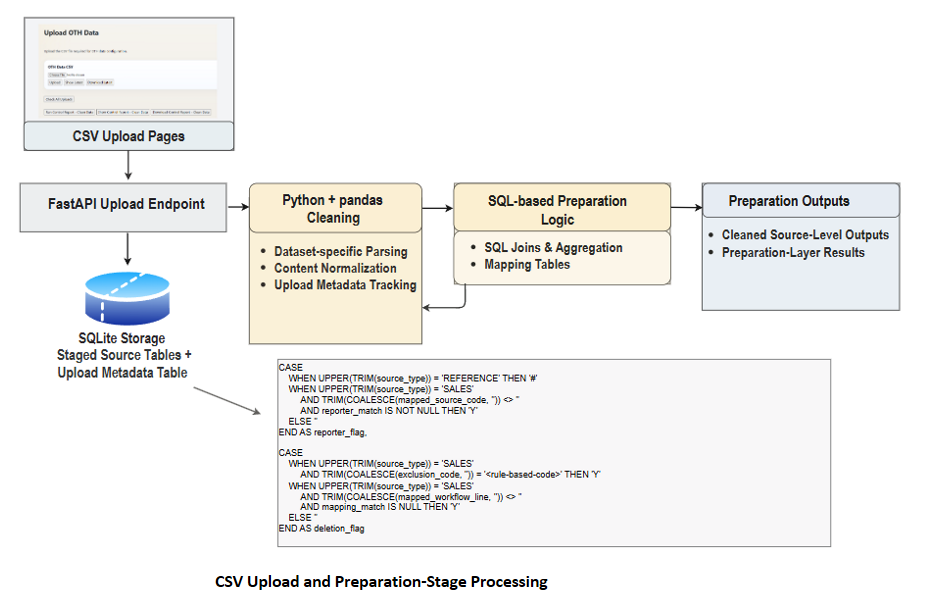
\includegraphics[width=1.1\linewidth]{5.4.png}
    \caption{Implementation of CSV upload and preparation-stage processing}
    \label{fig:appendix-upload-preparation}
\end{figure}

\begin{figure}[H]
    \centering
    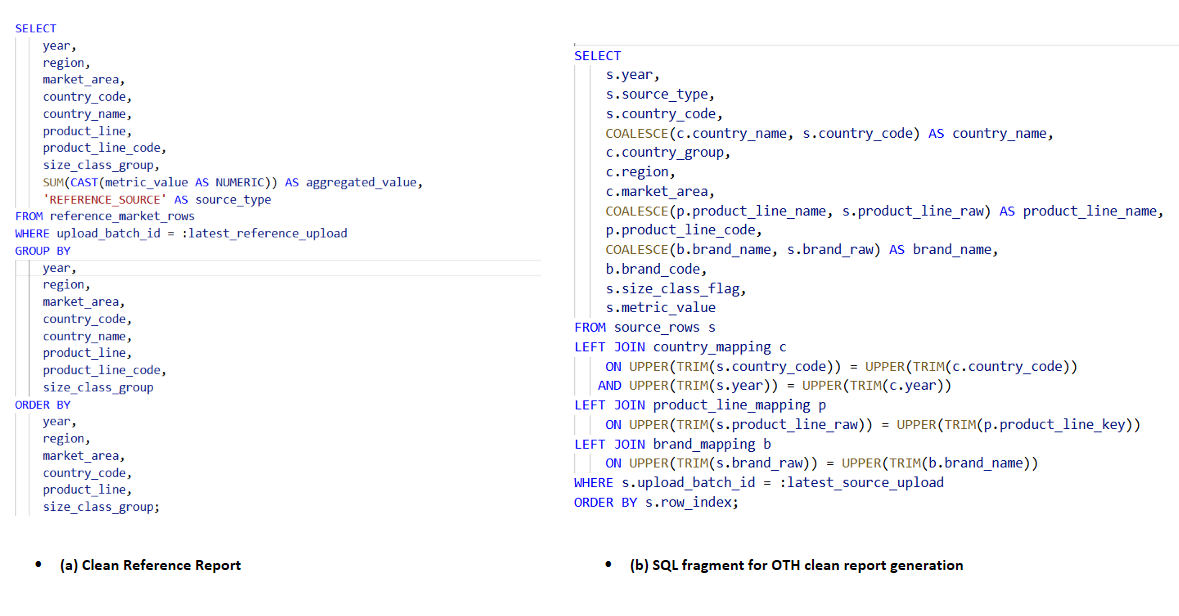
\includegraphics[width=1.1\linewidth]{5.4.1.png}
    \caption{Anonymised and simplified SQL fragments for CRP/TMA and OTH clean report generation}
    \label{fig:appendix-sql-preparation}
\end{figure}

The preparation stage follows the general execution pattern used throughout the prototype. A frontend workflow page triggers a FastAPI endpoint, which resolves the latest successful uploads, executes SQL transformations, and returns normalized rows as JSON for inspection. The same frontend-backend execution structure is reused in later workflow stages.

Adjustment-layer execution follows the same pattern, but the backend processing becomes more calculation-oriented. After the adjustment endpoint is triggered, the backend retrieves the prepared rows and executes grouped SQL queries that aggregate total-market and internal-sales values by shared workflow keys. These queries derive adjustment-layer values through conditional aggregation. The backend returns both source-detail rows and result rows, allowing the frontend to display not only the calculated output but also the data basis from which it was derived.

\begin{figure}[H]
    \centering
    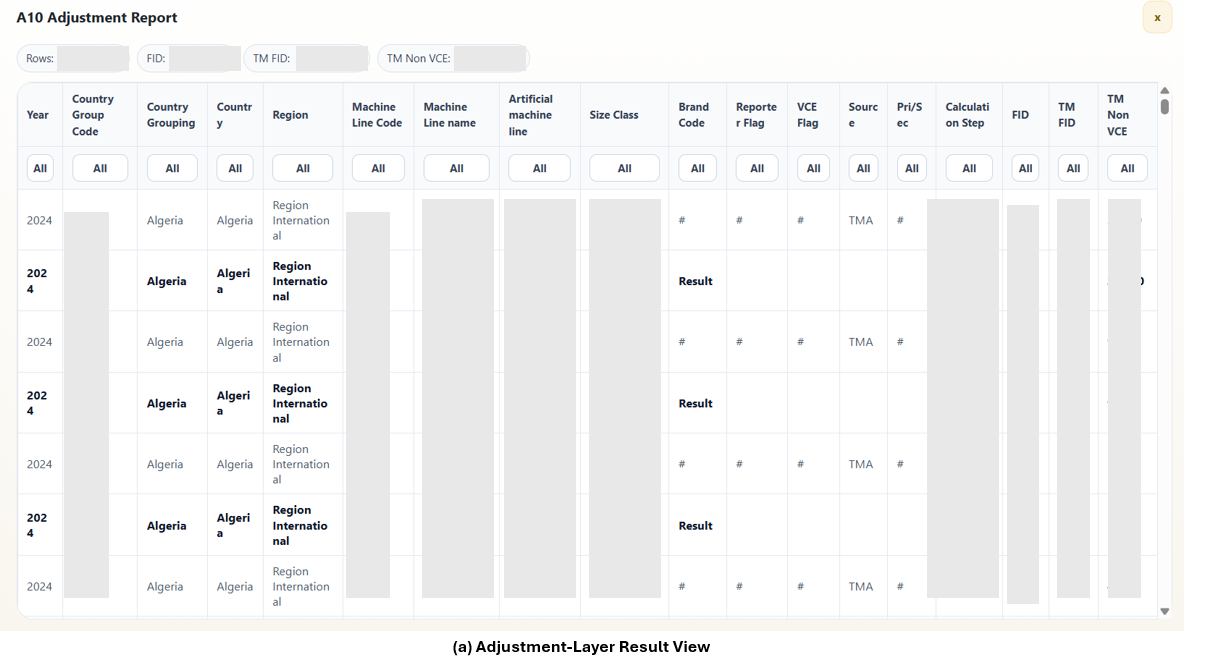
\includegraphics[width=1.1\linewidth]{5.6.1.1.png}
    \caption{Adjustment-layer result view}
    \label{fig:appendix-adjustment-view}
\end{figure}

\begin{figure}[H]
    \centering
    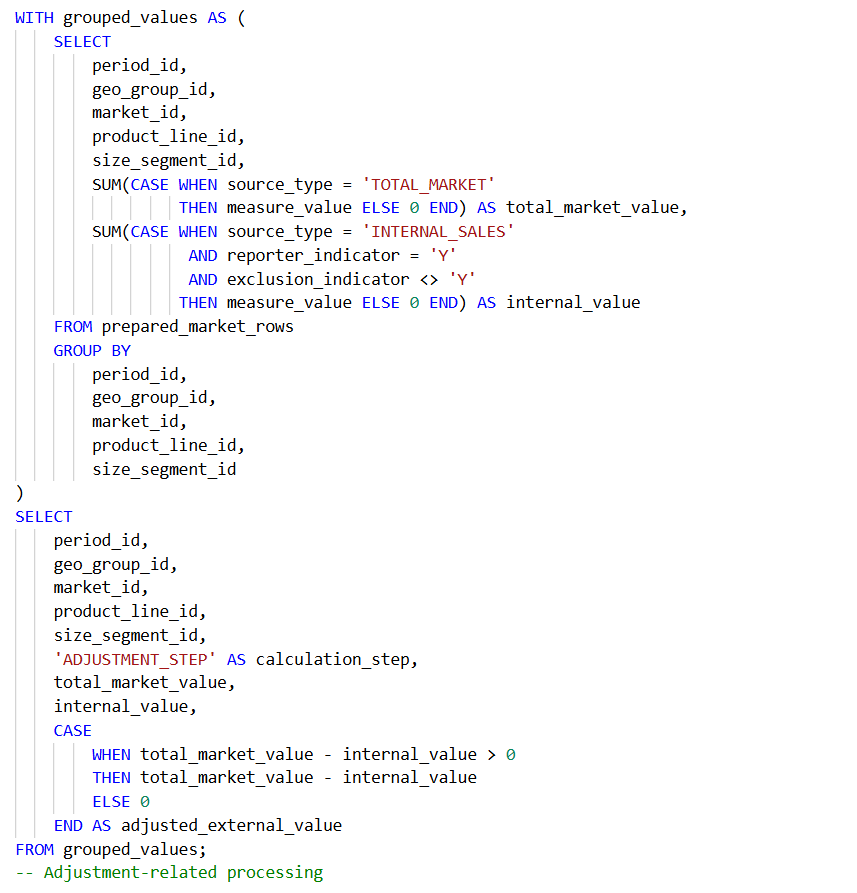
\includegraphics[width=1.1\linewidth]{5.6.1.1.1.png}
    \caption{Anonymised SQL fragment for adjustment-layer value calculation}
    \label{fig:appendix-adjustment-sql}
\end{figure}

The machine-line split stage uses a mixed execution model. SQL is used to prepare the required source and reference data, while Python is used for the redistribution calculation itself. When the user triggers a split-related report, the backend first resolves the latest required datasets and executes SQL logic to obtain eligible OTH rows and reference rows containing total-market non-VCE values. SQL therefore prepares the source rows, applies reporter and deletion logic, derives reference structures, and aggregates the values needed for proportional redistribution.

After the SQL preparation step, Python backend logic performs the split calculation. For each eligible OTH row, the backend determines the most appropriate reference level, such as country, region, or country grouping, and redistributes the input value according to the available non-VCE reference distribution. Formally, the redistribution can be expressed as:

\[
FID_{\text{split}, i}
=
FID_{\text{input}}
\times
\frac{TM_{\text{non-VCE}, i}}
{\sum_{j \in Targets} TM_{\text{non-VCE}, j}}
\]

where \(FID_{\text{input}}\) is the original OTH value to be redistributed, \(TM_{\text{non-VCE}, i}\) is the reference non-VCE value for target destination \(i\), and \(\sum_{j \in Targets} TM_{\text{non-VCE}, j}\) is the total reference non-VCE value across all valid target destinations in the same split group.

Once the calculation is completed, the backend constructs output rows containing source rows, split-result rows, supporting reference rows, split ratios, and before-after difference values. These outputs can either be saved as snapshots in the database or returned directly as JSON. The frontend then renders the results in workflow-specific inspection tables.

\begin{figure}[H]
    \centering
    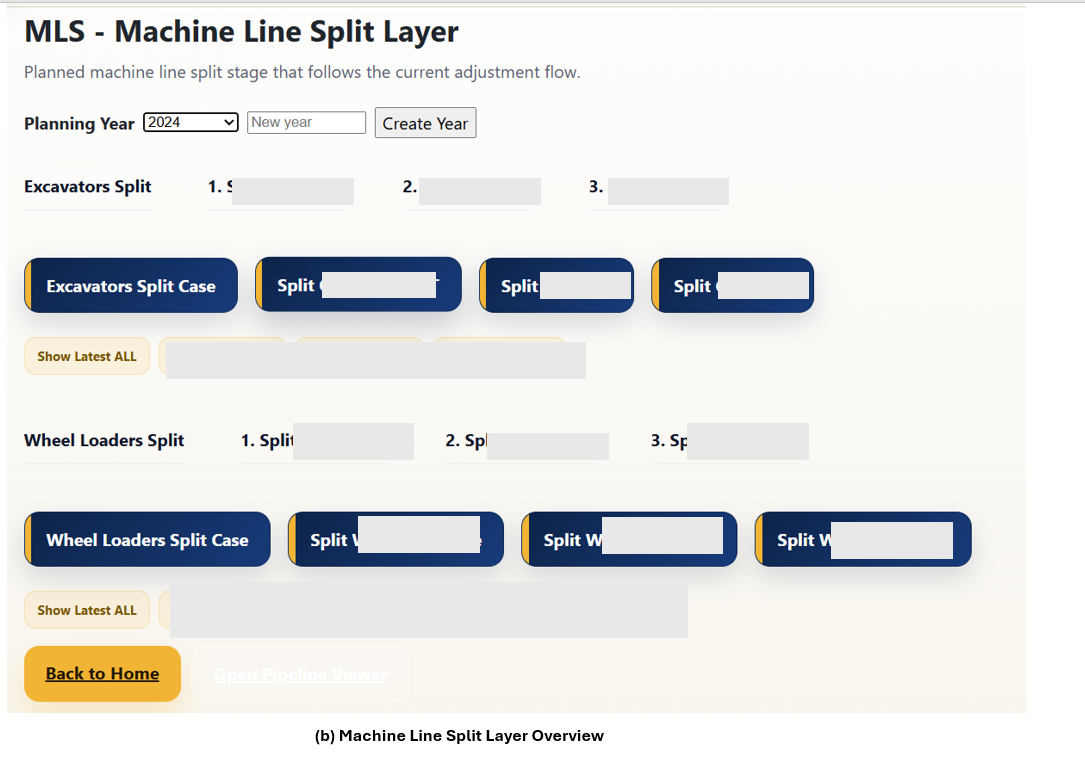
\includegraphics[width=1.1\linewidth]{5.6.1.2.png}
    \caption{Machine line split layer overview}
    \label{fig:appendix-split-overview}
\end{figure}

\begin{figure}[H]
    \centering
    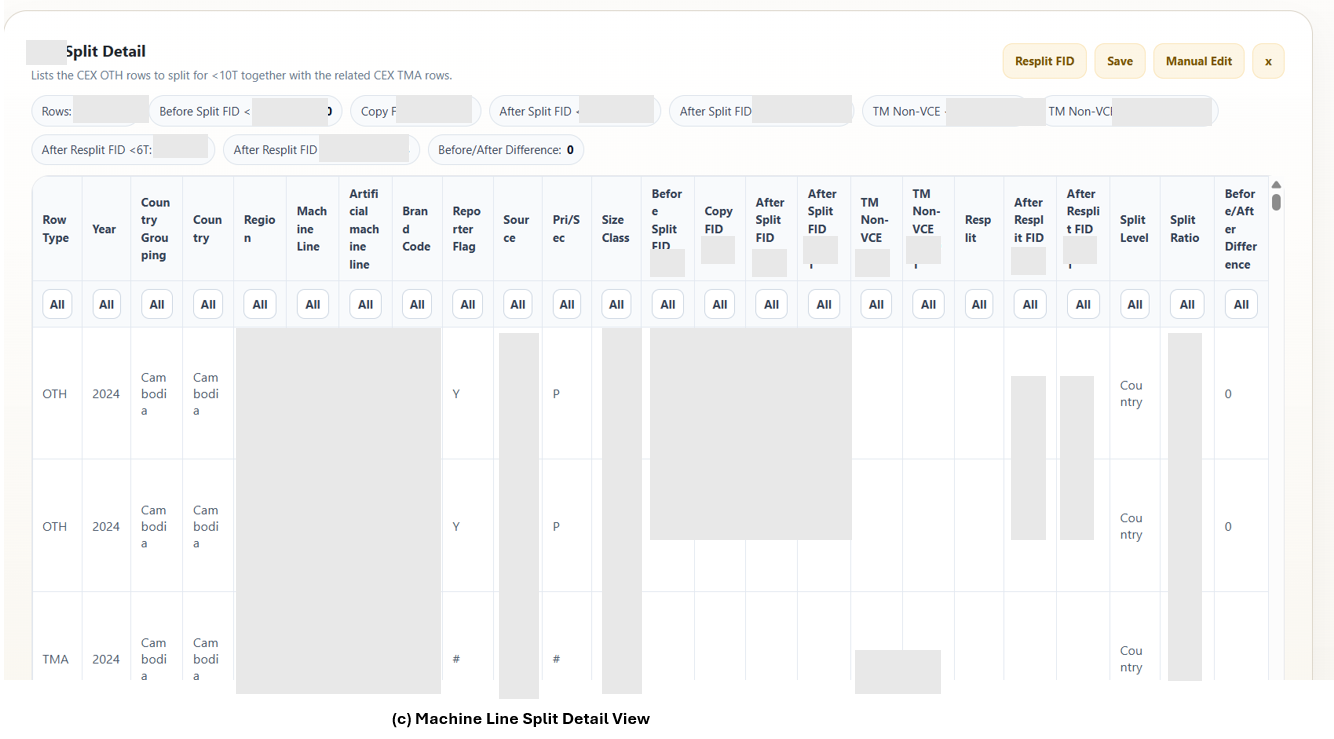
\includegraphics[width=1.1\linewidth]{5.6.1.3.png}
    \caption{Machine line split detail view}
    \label{fig:appendix-split-detail}
\end{figure}

\begin{figure}[H]
    \centering
    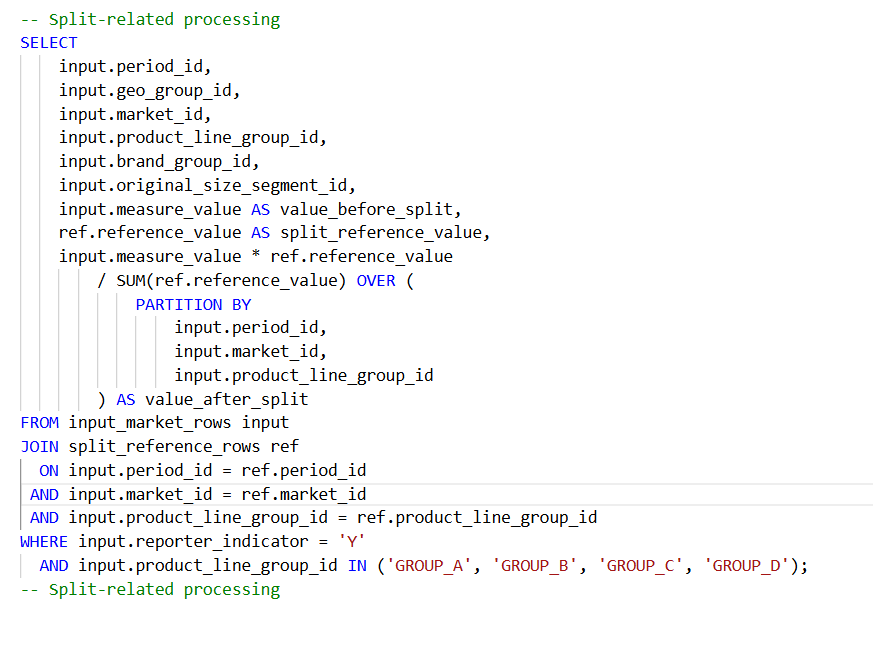
\includegraphics[width=0.85\linewidth]{5.10.png}
    \caption{Anonymised SQL and backend-processing fragments for adjustment- and split-related logic}
    \label{fig:appendix-sql-split}
\end{figure}

Frontend reporting views were developed in parallel with backend execution endpoints. They render structured JSON responses in workflow-specific inspection pages and support filtering, aggregation, and export. Overall, the implementation establishes a clear division of responsibility: the frontend triggers actions and visualizes outputs, SQL prepares and aggregates workflow data, Python handles more complex calculations such as split redistribution, and the backend returns or persists the resulting rows for later reuse.

\section{Detailed Requirement Evaluation}

The artefact was evaluated against the functional and performance requirements defined in Section~\ref{sec:requirements}. The evaluation used generated workflow outputs, SAP reference comparisons where applicable, manual Excel checks, runtime observations, repeated stability testing, and stakeholder feedback.

Stakeholder feedback was collected through weekly demo meetings and review discussions with Volvo CE stakeholders involved in the TMC workflow. During these meetings, prototype results and intermediate outputs were demonstrated, and the implemented rules were reviewed and confirmed with stakeholders. The feedback was reviewed in a qualitative and descriptive way to assess whether the separated workflow views, filters, summaries, and intermediate outputs improved practical transparency, inspectability, and usability. Manual Excel checks, output comparison, and runtime observations were used separately to assess rule correctness, validation support, and prototype performance.

\begin{longtable}{|>{\raggedright\arraybackslash}p{3.0cm}|>{\raggedright\arraybackslash}p{4.5cm}|>{\raggedright\arraybackslash}p{6.3cm}|}
\caption{Evaluation against functional and performance requirements}
\label{tab:evaluation_parameters} \\
\hline
\textbf{Requirement} & \textbf{Evaluation Question / Metric} & \textbf{Evidence and Result} \\
\hline
\endfirsthead

\hline
\textbf{Requirement} & \textbf{Evaluation Question / Metric} & \textbf{Evidence and Result} \\
\hline
\endhead

FR1 Functional fulfilment & Can required source and matrix files be uploaded, shown, downloaded, and reused? & Yes. The required datasets in scope were uploaded and reused in workflow execution, including Source Matrix, Reporter List, Size Class, Brand Mapping, Group Country, Machine Line Mapping, OTH, CRP- and TMA-related data, and Volvo CE sales data. Upload pages supported \textit{Show Latest} and \textit{Download Latest}, enabling users to review and retrieve the latest uploaded files. \\
\hline

FR2 Functional fulfilment & Can backend logic generate staged workflow outputs for the selected TMC stages? & Yes. The backend generated staged outputs for OTH deletion and reporter-base processing, preparation, market view, adjustment, and split/resplit. These outputs were used for later inspection, comparison, and validation against expected workflow logic. \\
\hline

FR3 Functional fulfilment & Does the artefact support a modular web-based frontend-backend workflow? & Yes. The prototype operated with separated frontend pages, backend report and processing routes, and relational storage for uploaded and derived records. Upload, processing, storage, workflow inspection, and visualisation were implemented as separate functions, supporting a modular workflow structure. \\
\hline

FR4 Functional fulfilment & Are uploaded files, mappings, workflow records, and generated outputs stored in a structured way for repeated review? & Yes. Uploaded files, mapping data, intermediate records, and generated outputs were stored and reused across stages. Repeated save and reload cycles confirmed that users could return to generated results and continue review without rerunning the whole workflow. \\
\hline

FR5 Transparency and traceability support & Are intermediate stages and relevant source/rule context inspectable? & Partly to fully. Stage outputs were visible separately, including OTH deletion base, preparation, adjustment, market view, and split/resplit. Outputs retained key context fields, including source, country, machine line, artificial machine line, brand, reporter/deletion flags, split level, and split ratio. This enabled stage-level tracing, although full end-to-end row-level lineage remains future work. \\
\hline

FR6 Usability and review support & Can users inspect outputs through frontend review functions? & Yes. Users reviewed outputs through filterable tables, summary cards, chart-based views, and CSV export. Stakeholder feedback indicated that the separated views and intermediate outputs made the selected TMC stages easier to inspect and discuss compared with the prior SAP-based representation. \\
\hline

FR7 Validation support & Do outputs support comparison with business rules, reference outputs, and manually checked results? & 
Mostly yes.
\begin{itemize}[leftmargin=*, nosep]
    \item Manual Excel filtering was used to verify whether prototype-generated reporter flags and deletion flags followed the predefined rule requirements. The manually checked Excel results matched the prototype outputs.
    \item CRP reporter rows also matched the SAP reference result, with 338 rows identified.
    \item For OTH, the prototype classified 3,452 reporter rows, while SAP contained 3,467 rows with a net FID difference of 68. This was traced to a reporter-list version difference rather than a prototype error.
    \item About 20\% of market-view rows and 10\% of split/resplit rows were spot-checked. The sampled records were consistent with expected calculations, split-case selection, redistribution logic, and before/after total preservation. One split-ratio discrepancy was recorded as a rule-clarification finding.
\end{itemize}
\\
\hline

FR8 Prototype environment and adaptability & Can the artefact run as a browser-based prototype and remain adaptable for future infrastructure? & Yes within the prototype scope. The system was evaluated as a browser-accessible prototype with frontend, backend service, and relational database using 2024 workflow data. The modular design supports future adaptation to cloud or Volvo CE internal infrastructure, although enterprise integration, production deployment, and internal authentication constraints remain future work. \\
\hline

PR1 Performance & Can the 2024 workflow be completed within the defined 40-minute review window? & 
Yes. The selected 2024 workflow was tested \textbf{five} times and completed within the defined \textbf{40-minute} review window.
\begin{itemize}[leftmargin=*, nosep]
    \item Matrix upload: approximately \textbf{4--5 minutes}
    \item OTH and CRP data upload: approximately \textbf{5 minutes in total}
    \item Preparation: approximately \textbf{10 minutes}
    \item Adjustment: approximately \textbf{3 minutes}
    \item Machine line split: approximately \textbf{10--12 minutes}
\end{itemize}
The total measured time was approximately \textbf{32--35 minutes}, including processing, result inspection, manual correction, and saving of outputs.
\\
\hline

PR2 Performance and stability & Is behaviour stable during repeated upload, run, filter, save, reload, and export cycles? & 
Yes. The prototype was tested through \textbf{five} repeated operation cycles using the selected 2024 dataset.
\begin{itemize}[leftmargin=*, nosep]
    \item Each cycle covered matrix upload, OTH/CRP upload, preparation, adjustment, machine line split, filtering, manual correction, saving, reload, and CSV export.
    \item The average full workflow cycle was approximately \textbf{33 minutes}.
    \item No crash, data loss, or inconsistent save/reload behaviour was observed.
\end{itemize}
\\
\hline

\end{longtable}
